\section{Background and Observations}

In this section, we first study the typical shuffle characteristics (\ref{shuffle pattern}), and then spot the opportunities to achieve shuffle optimization (\ref{observation}).
\subsection{Characteristic of Shuffle} \label{shuffle pattern}

In large scale data parallel computing, shuffle is designed to achieve an all-to-all data blocks transfer among nodes. For a clear illustration, we use \textit{map tasks} to define the tasks that generate shuffle data and use \textit{reduce tasks} to define the tasks that consume shuffle data.
% Note that one task may have both shuffle data generation and consumption in modern DAG framework. These tasks contain characteristic of both map task and reduce task. But these tasks won't change the behavior of shuffle. To avoid ambiguity, in the following paper, we will only use term of map task to represent those who produce shuffle output, and reduce task to represent those who consume shuffle output.
% \begin{figure}
% 	\centering
% 	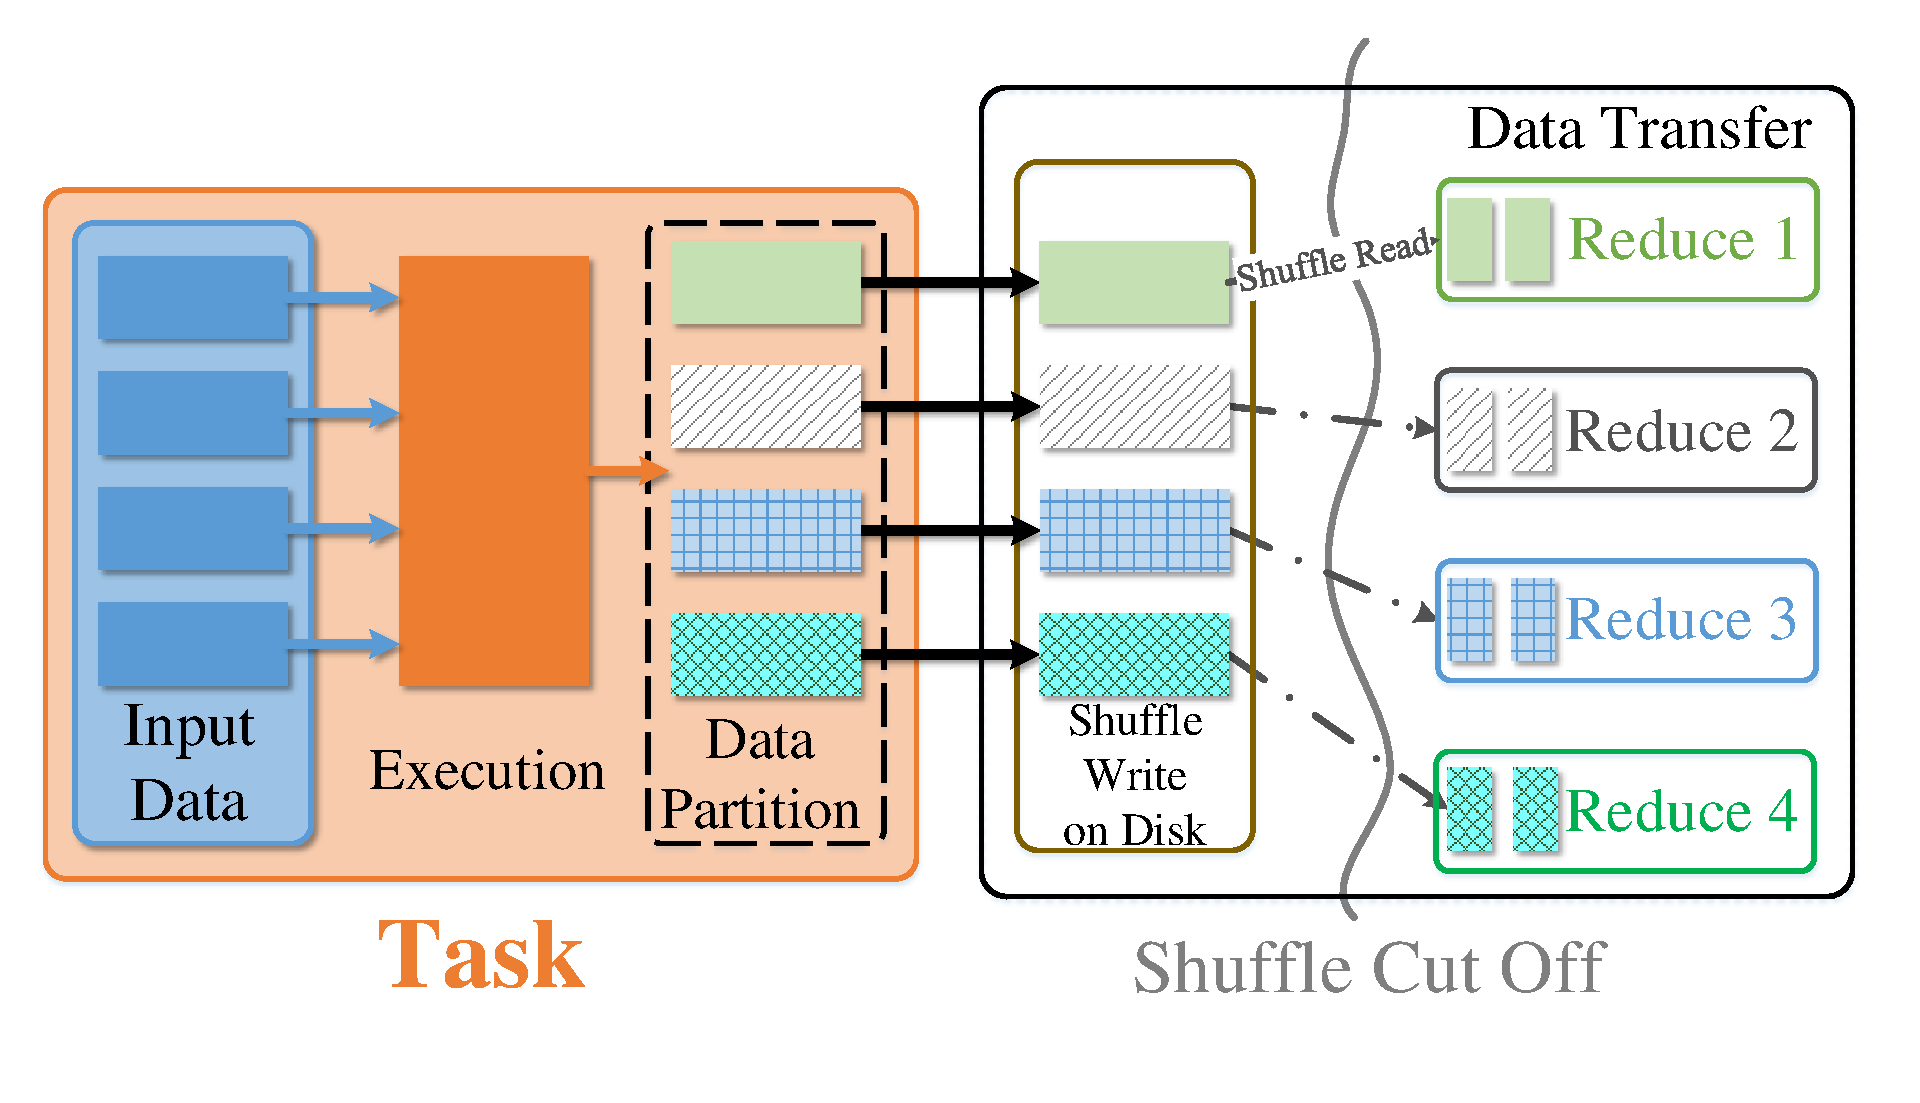
\includegraphics[width=\linewidth]{fig/shuffle_process}
% 	\caption{Shuffle Overview}
% 	\label{fig:shuffle_process}
% \end{figure}

\textbf{Overview of shuffle process}. Each map task partitions the result data (key, value pair) into several buckets according to the partition function (e.g., hash). The total number of buckets equals the number of tasks in the next step.
% shuffle data is produced by \textit{data partition}. For \textit{data partition}, 
Shuffle can be further split into two parts: \textit{shuffle write} and \textit{shuffle read}. 
The partitioned shuffle output data will be spilled to local persistent storage during shuffle write.
Shuffle read starts at the beginning of reduce tasks. It fetches data as reduce input from both remote and local storage.

\begin{figure}
	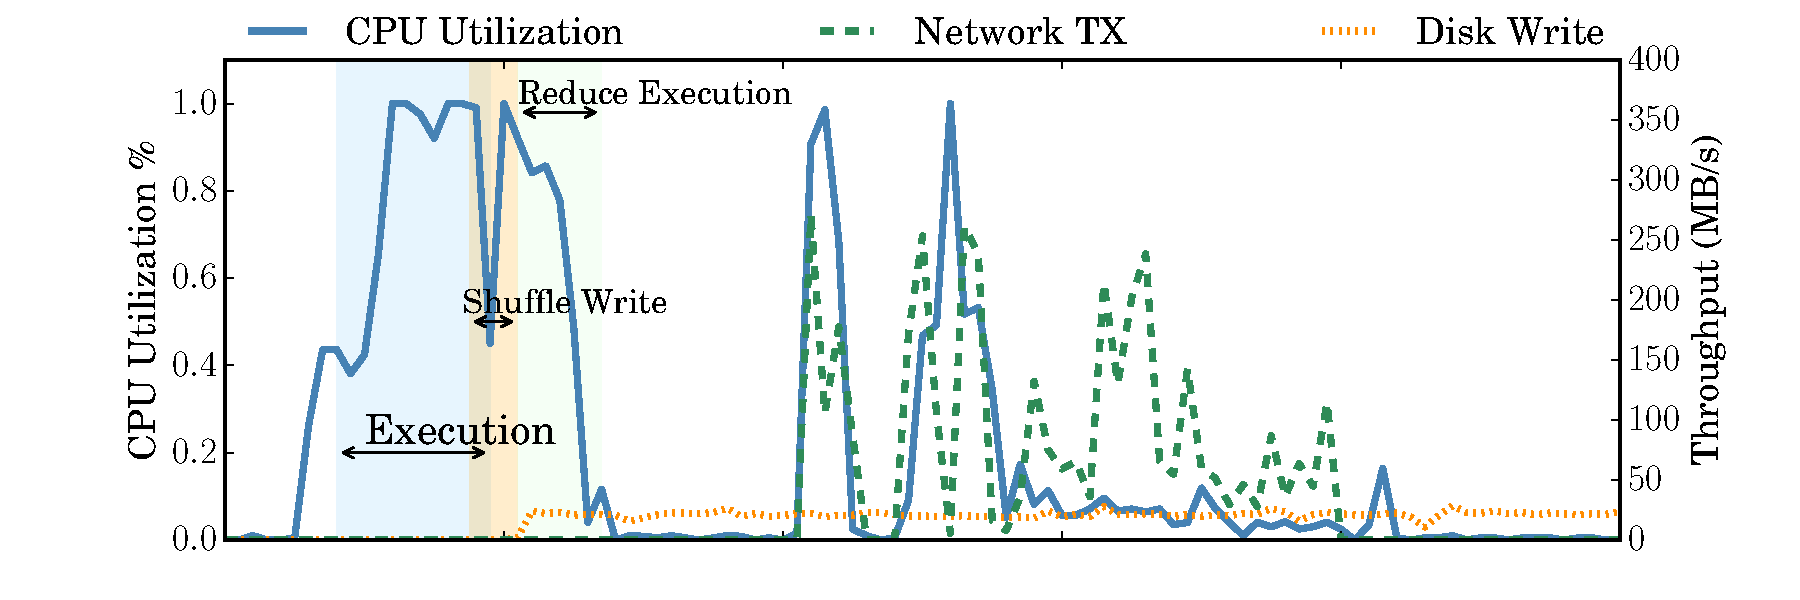
\includegraphics[width=\linewidth]{fig/util}
	\caption{CPU utilization and I/O throughput of a node during a Spark single shuffle application}
	\label{fig:util}
\end{figure}
%In short, shuffle is loosely coupled with application context and it's I/O intensive.

\textbf{Impact of shuffle process}. Shuffle process is I/O intensive, which might introduces a significant latency to the application. Reports show that 60\% of MapReduce jobs at Yahoo!
and 20\% at Facebook are shuffle intensive workloads \cite{shufflewatcher}. For those shuffle intensive jobs, the shuffle latency may even dominate Job Completion Time (JCT).
For instance, a MapReduce trace analysis from Facebook shows that shuffle accounts for 33\% JCT on average, up to 70\% in shuffle intensive jobs \cite{managing}.
% Besides, the completion time of shuffle correlates with the performance of storage devices, network and even applications.
% This variation may bring a huge challenge for operators to find the correct configuration of the DAG framework.


\subsection{Observations} \label{observation}
Of course, shuffle is unavoidable in a DAG computing process. But can we mitigate or even remove the overhead of shuffle? To find the answers, we run some typical Spark applications in a 5-node EC2 cluster with \texttt{m4.xlarge}. We then measure the CPU utilization, I/O throughput, and tasks execution information of each node. Here we present the trace of one node running Spark \textit{GroupByTest} in Figure \ref{fig:util} as an example. This job has 2 rounds of tasks for each node.
We have marked out the \textit{execution} phase as from the launch time of the first task to the execution finish timestamp of the last one. The \textit{shuffle write} phase is marked from the timestamp of the beginning of the first partitioned data write. The \textit{shuffle read and execution} phase is marked from the start of the first reduce launch timestamp.

% Figure \ref{fig:util} reveals the performance information of two stages that are connected by shuffle. By analyzing the trace with Spark source code \cite{sparksource}, we propose the following observations.
% \begin{figure*}
% 	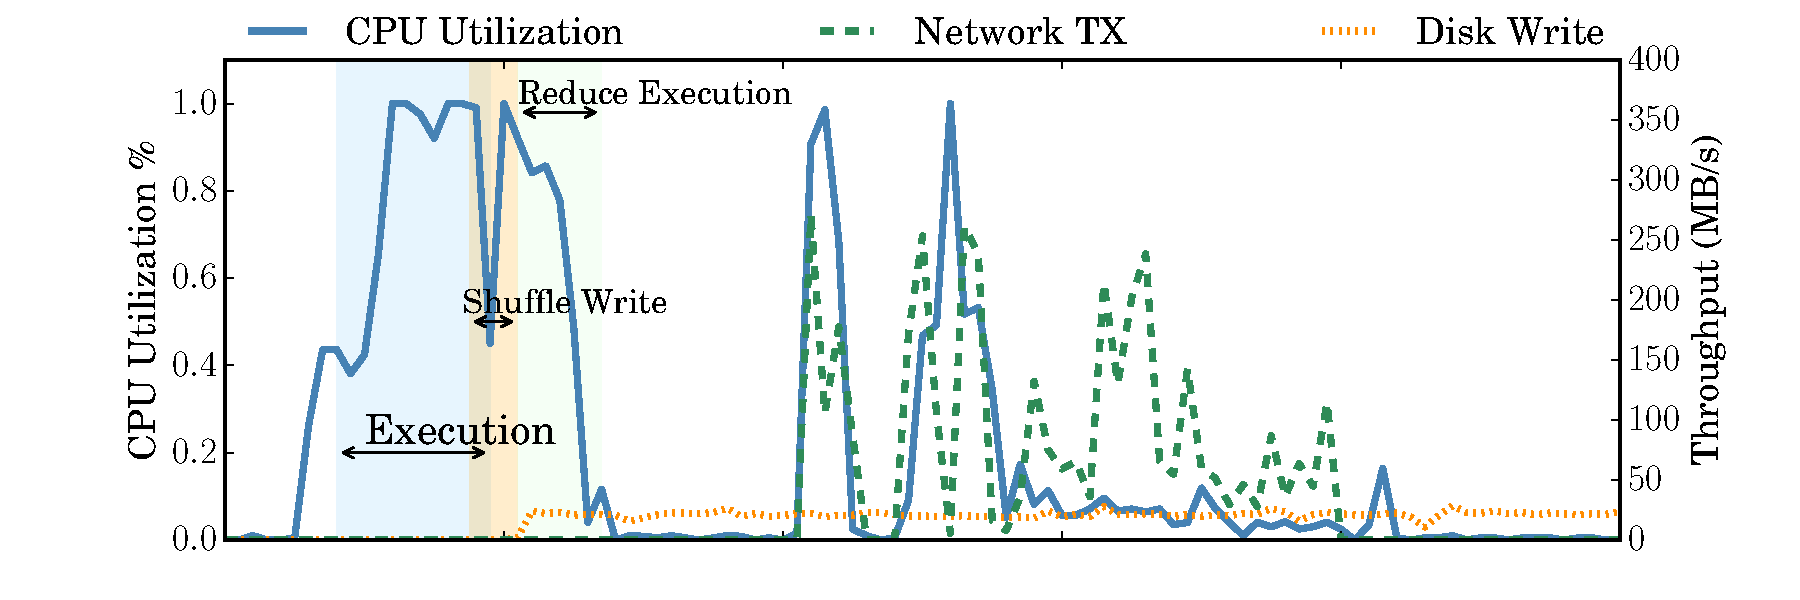
\includegraphics[width=\textwidth]{fig/util}
% 	\caption{CPU utiliazation and I/O throughput of a node during a Spark single shuffle application}
% 	\label{fig:util}
% \end{figure*}


\subsubsection{Coarse Granularity Resource Allocation}
In Figure \ref{fig:util}, when a slot is scheduled to a task, it will not be released until the the task completes \textit{shuffle write}. On the reduce side, the network transfer of shuffle data introduces an explicit I/O delay during \textit{shuffle read}. Meanwhile, shuffle is I/O intensive. Both \textit{shuffle write} and \textit{shuffle read} occupy the slot without involving much CPU. The current coarse slot --- task mapping results in an inconsistency between resource demands and slot allocation thus decreases the resource utilization. To break this inconsistency, a finer granularity resource allocation scheme must be provided.

\subsubsection{Synchronized Shuffle Read}
Almost all reduce tasks start \textit{shuffle read} simultaneously. The synchronized \textit{shuffle read} requests cause a burst of network traffic. As shown in Figure \ref{fig:util}, the data transfer stresses on network bandwidth, which may results in network congestion and further hurts the performance of reduce stage.
% The previous work \cite{coflow, managing} also proves that the network transfer can introduce significant overhead in DAG computing.

\subsubsection{Inefficient Persistent Storage Operation}
At first, both shuffle write and read are tightly coupled with task execution, which results in a blocking style I/O operations. This blocking I/O operation along with synchronized shuffle read may introduce significant latency, especially in a I/O performance bounded cluster.
Besides, the legacy of spilling shuffle data to disk directly is too conservative in modern cluster with large memory. Compared to input dataset, the size of shuffle data is relatively small. For example, shuffle size of Spark Terasort \cite{spark-tera} is less than 25\% of input data. The data reported in \cite{makingsense} also shows that the amount of data shuffled is less than input data, by as much as 10\%-20\%. On the other hand, numbers of memory based distributed storage system have been proposed \cite{memcached, tachyon, ramcloud} to move data back to memory. 
We argue that the memory capacity is large enough to store the short-living shuffle data with cautious management.

\subsubsection{Multi-round Tasks Execution}\label{multi}
Both experience and DAG framework manuals recommend that multi-round execution of each stage will benefit the performance of applications.
For example, Hadoop MapReduce Tutorial \cite{hadooptutorial} suggests that \textit{10-100 maps} per-node and \textit{0.95 or 1.75 $\times$ no. of nodes $\times$ no. of maximum container} per-node seem to be the right level of parallelism. Spark Configuration also recommends $2-3$ tasks per CPU core in the cluster \cite{sparkconf}.
Since the shuffle data becomes available as soon as the end of map task execution. At the same time, the network is idle during the map stage (network utilization during map stage in Figure \ref{fig:util}). If the destination host of the shuffle data can be predicted in priori, the property of multi-round can be leveraged to overlap the \textit{shuffle read} operation.
% There are at least two persistent storage operations for each shuffle data block. At first, Spark will write shuffle data to the persistent storage after map task execution (i.e. \textit{shuffle write} in Figure \ref{fig:util}). During the \textit{shuffle read}, Spark will read shuffle data from remote and local persistent storage, which is the second operation. The persistence of shuffle data was designed for fault tolerance. But we believe it is not necessary for today's cluster. Recall that shuffle data only exist in a short time scale. But the Mean Time To Failure (MTTF) for a server is counted in the scale of year \cite{tachyon}, which is exponential compared with the duration of a shuffle. In addition, the capacity of memory and network has been increasing rapidly in recent years. As a result, numbers of memory based distributed storage system have been proposed \cite{memcached, tachyon, ramcloud}. On the other hand, the size of shuffle data is relatively small. For example, shuffle size of Spark Terasort \cite{spark-tera} is less than 25\% of input data. The data reported in  \cite{makingsense} also shows that the amount of data shuffled is less than input data, by as much as 10\%-20\%. We argue that removing persistent storage and using memory to achieve shuffle fault tolerance is feasible and efficient.

Based on these observations, it is straightforward to come up with an optimization that starts shuffle read ahead of reduce stage to overlap the I/O operations in multi-round of DAG computing tasks and uses memory to store the shuffle data to further decrease shuffle overhead. To achieve this optimization:
\begin{itemize}
	\item Shuffle process should be decoupled from task execution to achieve a fine granularity scheduling scheme.
	\item Reduce tasks should be pre-scheduled without launching to achieve shuffle data pre-fetching.
	\item Shuffle process should be taken over and managed outside DAG frameworks to achieve a cross-framework optimization
\end{itemize}
In the following section, we elaborate the methodologies to achieve three design goals.
